
%Prepare the tests on the EPICEA active sub-system (to be subcontracted)
%- Develop the active EPICEA sub-system for a SRAM-based CR emulation strategy for complex systems. Use
%of FPGA circuits from Xilinx allowing CR emulation (without CR illumination) by bit flipping for preparing
%the tests to be performed by the CR test subcontractor

\section{Context and Motivation}
\label{intro}

This thesis is part of a wider project, called EPICEA (Electromagnetic Platform for lightweight 
Integration/Installation of electrical systems in Composite Electrical Aircraft), in collaboration with several 
companies and agencies (Bombardier, Isoneo, ARTTIC, ONERA, AXESSIM, FOKKER ELMO BV, IDS). The EPICEA project will approach
numerous avionic engineering design issues in the advancement of future aircraft, aiming at a significant
reduction of energy consumption through more electrical aircraft and systems integration. The EPICEA project strives to understand the electromagnetic (EM) issues on composite electric aircraft (CEA). This includes the analysis
and characterization of EM coupling, interconnects, and cosmic radiations (CR) on electrical systems together
with new concepts of antennas design to maintain performance in a composite environment without modifying
aircraft aerodynamics.

This thesis contribution to the EPICEA project is "the study of CR effects on aircraft electrical systems based on the reconfigurable fabric, e.g., Field Programmable Field array (FPGA)." This research work focuses on extraction of the faulty response (signature) from the sequential digital circuit from the FPGA-based platform to help to investigate the effects of CR on an embedded electronic system of the aircraft and to model and analyze the faulty behavior of the sequential digital circuits. This thesis aims to make the high-level fault model that will use to investigate the effects of radiation on the aircraft flying at the altitude of 50,000 feet or above. This thesis helps to find; at high altitude when aircraft gets more exposure to the radiation the reliability of the FPGA based embedded systems is a primary concern; the phenomena causing faults in the FPGA based embedded systems should be studied in a way to know early in the embedded electronic design of the aircraft if mitigation strategies are required to deal this higher radiation level. 

In order to accomplish our tasks, we need to understand the space radiation environment which has two preliminary sources --- galactic cosmic radiation and solar energetic particles~\cite{SWE20216}. The galactic cosmic radiation from outside the solar system consists mostly of energetic protons and heavy ions, e.g., iron. Solar energetic particles are commonly associated with the solar flare events and primarily dominated by the proton.  The space radiation is an unavoidable space weather phenomena. This research thesis is solely concern with the aircraft flying at the altitude of 50,000 feet or above, where the vulnerability of the circuit is due to the neutrons~\cite{xilinnseu}. The cosmic rays are originating in outer space and travel at nearly the speed of light and strike the earth from all directions. These cosmic radiations are ranging from lightest to heaviest elements in the periodic table. When these high-energy cosmic rays interact with the earth's magnetosphere, neutrons are generated, often referred to as an air shower~\cite{lesea2005rosetta}.  An intense neutron environment exists at higher altitudes in the atmosphere, 10 km to 40 km.  Long-haul aircraft are flying at the altitudes of 50,000 feet nearly 15 km at the latitude of \ang{60} under the influence of greatest neutron flux approximately 500 times that a ground-based observer in Newyork City~\cite{lesea2005rosetta}. When these neutrons interact with the semiconductor, e.g., silicon they can produce secondary particles if these secondary particles are charged and they can generate the trails of an electron-hole pair of a few microns in length and if this trail happens near the PN-junction in a transistor, a voltage spike can generate. This voltage spike is enough to change the state of a memory cell or flip-flop, results in a drastic consequence and cause Single Event Upsets (SEUs) also called soft-error in SRAM-based FPGAs. The impact and implications of the soft-errors due to the interaction of neutrons with the avionics embedded system are now recognized as an area of active research. Especially, the incident happened with the Qantas Flight Airbus A330-303 flying from Singapore to Perth went under the two terrifying dives due to the malfunction of the on-flight computer. After, the investigation it revealed that high-energy particles from the outer space --- were the responsible for the malfunction of the computer. And, the potential triggering event was the single-event effect (SEE) interacting with one of the integrated circuits (ICs) within the CPU module. 




%
%The Neutrons are generated in the atmosphere when cosmic rays in the outer space, strike Earth from all the direction. When these neutrons interact with the semiconductor e.g., silicon they can generate secondary particles, if these secondary particles are charged and they are able to generate the trails of electron-hole pair of a few microns in length and if this trail happens near the PN-junction in a transistor, a voltage spike can generate. This voltage spike is enough to change the state of a memory or flip-flop.

Therefore, fault management strategies are essential to apply on the aircraft's embedded systems. Before need to know to apply the mitigation techniques early in the embedded electronic design, if we know the high-level fault model of the FPGA-based circuits at high-level of abstraction that facilitate without going into the detailed simulation get the faulty behavior of the component at high-level.

  

\section{Problem Statement}

A soft error will occur when a radiation event causes enough charge disturbance to flip the state of a logic gate, memory element, or flip-flop. The soft errors are also referred as radiation-induced faults, e.g., neutrons from the cosmic rays. The fault caused by the SEUs have implications on the behavior of the system. However, the soft errors do not break the silicon but can corrupt the underlying functionality and produce severe consequences if they are successfully propagated to the primary outputs or stored by the memory cell. In this work, we will evaluate the faulty behaviors of the sequential circuit, given the faulty sequential circuit behavior, and model it to the high-level of abstraction. We want to make the high-level fault model to see the severity of the faulty behavior induced by the SEUs.


%\begin{figure}
% \centering
%  \captionsetup{justification=centering}    
%   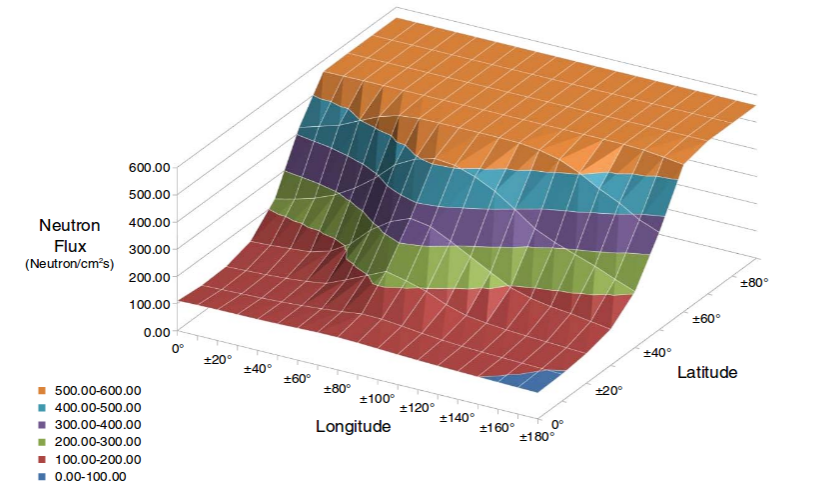
\includegraphics[scale=0.4]{figures/img/neutron-flux.png}
%   \caption{Neutron Flux at 40,000 Feet.}
%\label{fig:neu-flux}
%\end{figure}





\section{Research Objectives}



In this thesis, I propose a methodology for modeling the faulty sequential circuits to model the output of the soft error problem at a behavioral level. We will use the high-level modeling techniques, e.g., Markovian-system analysis to model the faulty behavior of the sequential circuits. The faulty behavior model is based on the analytical expression for modeling the signature (circuit fault response) from the experimental data generating by performing fault emulation on the FPGA. In this work, a novel approach will introduce to analyze the fault origination and propagation in the case of faulty sequential circuits, and will develop new models that can accurately see the severity of the faulty behavior from the signatures of the faulty circuits. The objectives of the present Ph.D. thesis are explained below: 

\begin{itemize}


\item{The main objective of this thesis is to develop a faulty behavior model for FPGA-based
sequential circuits described at a high-level of abstraction. The main purpose of developing a behavioral fault model of a circuit is to generate a library of faulty components reusable at high-level of abstraction}.



\item{The model has the capability to produce the faulty output of a circuit, and the probability of occurrence of faults.}

\item The model is to find the severity of a faulty behavior of the sequential circuit. 

\item The model is used for the signature analysis for the sequential circuit.
\item{Develop the faulty behavior model of different circuit
components, such as counter and FIR filter, using the high-level modeling technique.}

\item{Develop a library of the faulty behavior model of the sequential circuit
components comprising a Simulink model. So, each time designers need to analyze potential faulty behavior of a circuit at a high-level of abstraction, designer can utilize the faulty components from the library}.

\item Study the system susceptibility under neutron-induced single event effect.


%
%\item{The developed models could be used to
%replace any component of the entire circuit with faulty versions of the components described
%at a high-level of abstraction. The purpose of doing so to ensure that the effect of faulty behavior of each
%component on a system could be analyzed at a high-level of abstraction and the mitigation
%technique could be used to improve the robustness of critical parts of the design.}
%
%
%\item{The model will have the capability to compute the signature, also provide the worst-case input test vector, which has the highest probability to generate the faulty output, for any given sequential circuit. The model for sequential logic will have the ability to measure the maximum and average signature probabilities to construct a novel probabilistic model.}
%
%\item{Develop an abstraction of hardware signature that can be integrated into the high-level model, e.g., Simulink models.}
%
%\item{The goal of this research is to develop an approach for modeling the faulty behavior of a
%digital sequential circuit in the presence of the fault injection. The concept behind the fault injection process is to accelerate the occurrences of the signatures in the system to evaluate its functional behavior under the influence of expected faults on the
%FPGA-based systems.}





\end{itemize}




\subsection{Challenges}
Inorder to to achieve the above mentioned objectives. The main challenges we foresee are:
\begin{itemize}

\item Make a model at higher-level of abstraction from the data extracted at a lower level that represent the behavioral model of the respective signatures.
\item Develop a flow to convert faulty behavioral response of a sequential circuit into respective high-level model. This flow will be extensively validated by exhaustive fault emulation of ITC'99 benchmark. Develop a  fault behavioral model of different sequential circuits, e.g., counter, and FIR filter.

\item Develop a relationship between the bit-flip and the fault-model.

\end{itemize}


  

\section{Contribution}


This research thesis proposes a fault behavior model develop with the modeling techniques, e.g., Markovian-analysis in a novel way (utilize hidden Markov model (HMM) to represent faulty behavior of the sequential circuits). The Markovian system analysis will use to synthesize the faulty output of a circuit at high-level of abstraction. The existing faulty behavior model of the sequential circuits are not accurate as mostly models were based on simulation and on fault occurrence assumption.


\begin{itemize}

%\item In this work, we will construct a high-level fault model that model the signature of the sequential circuits (ITC'99 benchmark). The high-level behavioral model based on the signatures from the sequential circuits.

\item This work will focus on the soft-error susceptibility for sequential circuits which are different from the combinational circuits. The error in the sequential circuit can be propagated back to the inputs, or circuits outputs can be affected for several consecutive clock cycles making the design more vulnerable.  
\item Our model will have the capability can efficiently model the worst case signature and the input vector correlated with this signature, through probabilistic modeling (HMM) and have the ability to measure the maximum and average signature probabilities. We also try to establish a relationship between the FPGA bits emulation information to the faulty models.


\item We will propose the fault specific mitigation technique for handling soft-errors.
\end{itemize}

%%% Local Variables:
%% mode: latex
%% TeX-master: "../Document"
%% End:



